\section{$\qgr R$の定義}

以下$R$を可換環とする.
\begin{defn}
$\A$ をアーベル圏,$\B \subset \A$ を Serre 部分圏とする.すなわち,$\B$ は次の条件を満たす:
\begin{itemize}
  \item 任意の短完全列
  \[
  0 \to X \to Y \to Z \to 0.
  \]
  が $\A$ にあり,$Y$ が $\B$ に属するとき,$X$ および $Z$ も $\B$ に属する(逆も同様).
\end{itemize}
このとき,$\B$ による $\A$ のSerre 商圏(Serre quotient category)$\A/\B$ は次のように定義される:
\begin{itemize}
  \item 対象は $\A$ の対象と同じである.:
		\[\Ob(\A/\B)\coloneq \Ob(\A).\]
  \item 射は以下のように定義される:
  \[
  \Hom_{\A/\B}(X, Y) := \varinjlim_{\substack{X' \subset X\\ X/X' \in \B}} \varinjlim_{\substack{Y' \subset Y\\ Y' \in \B}} \Hom_{\A}(X', Y/Y').
  \]
\end{itemize}
\end{defn}

\begin{defn}[次数付き環]
環 $R$ が,アーベル群としての直和
\[ R = \bigoplus_{i \in \mathbb{Z}} R_i. \]
に分解され,かつ,環の積が任意の $i, j \in \mathbb{Z}$ に対して
\[ R_i R_j \subseteq R_{i+j} .\]
をみたすとき,$R$ を次数付き環 (graded ring) という.
このとき,$R_i$ の元を次数 $i$ の斉次元 (homogeneous element of degree $i$) と呼ぶ.
\end{defn}
以降,特に断りのない限り,次数付き環はネーター環であり,$R_0$ 上有限生成であるものとする.

\begin{defn}[次数付き加群]
$R = \bigoplus_{i \in \mathbb{Z}} R_i$ を次数付き環とし,$M$ を右 $R$-加群とする.
$M$ が部分加群の直和
\[ M = \bigoplus_{i \in \mathbb{Z}} M_i. \]
と表され、かつ、任意の $i, j \in \mathbb{Z}$ に対して、環の作用が
\[ R_i M_j \subseteq M_{i+j} .\]
をみたすとき、$M$ を次数付き$R$-加群 (graded $R$-module) という。
このとき、$M_i$ の元を次数 $i$ の斉次元 (homogeneous element of degree $i$) と呼ぶ。
\end{defn}
	
\begin{defn}
	 \( R = \bigoplus_{i \ge 0} R_i \)を次数付き環,\( M \in \gr R \)を$R$上の次数付き加群とする. $M$の元\( x \in M \) に対して,ある整数 \( i \gg 0 \) が存在して,\( R_{\ge i} \cdot x = 0 \) となるとき, 捻れ元(torsion element) であるという.ここで \( R_{\ge i} = \bigoplus_{m \ge i} R_m \) とする.

すべての元 \( x \in M \) が捻れ元である加群 \( M \)のことを捻れ加群(torsion module) であるという.このような加群全体のなす充満部分圏を \(\tors R\) で表す.
\end{defn}

\begin{prop}
次数付き環 \( R = \bigoplus_{i \ge 0} R_i \) に対し,その上の次数付き右$R$-加群全体のアーベル圏 \(\gr R\) において,torsion 加群全体からなる部分圏 \(\tors R\) は Serre部分圏である.
\end{prop}

\begin{defn}\cite{AZ94}
\(
R = \bigoplus_{i \ge 0} R_i
\) を次数付きネーター$\CC$-代数とする.\vspace{-3mm}
\begin{itemize}
  \item $\gr R$ は $\mathbb{Z}$-次数付き有限生成$R$-加群のアーベル圏とする.
  \item $\tors R$ は $\gr R$ のうち,ねじれ加群全体とする.
  \item $\qgr R$ は $\gr R$ の Serre 部分圏 $\tors R$ による商圏:$\qgr R := \gr R / \tors R$ と定義する.
\end{itemize}
\end{defn}

\begin{defn}\cite{GL87}
重み付き射影直線(weighted projective line)とは,以下のデータによって定まる射影曲線である:

\begin{itemize}
  \item 正の整数からなる列 $A = (a_0, a_1, \dots, a_r)$,
  \item $\mathbb{P}^1(k)$ の互いに異なる点の列 $\Lambda = (\lambda_0, \lambda_1, \dots, \lambda_r)$,
\end{itemize}

ただし,通常 $\lambda_0 = \infty,\ \lambda_1 = 0,\ \lambda_2 = 1$ と正規化する.次に,アーベル群
\[
	L_{A} \coloneq \ZZ \vec{x_1}\oplus\cdots\oplus\ZZ \vec{x_r}\oplus \ZZ\vec{c}\Big{/}\langle\vec{c} -a_i\vec{x_i}\mid i=1,\ldots,r\rangle.
\]
を定義し,これを次数付き群とする.多項式環: 
\[
	S = k[X_0, X_1, \dots, X_r], \quad \deg X_i = \vec{x}_i. 
\]
において,以下の $L_A$-斉次イデアル:
\[
	I_{A,\Lambda} = \left( X_i^{a_i} - X_1^{a_1} + \lambda_i X_0^{a_0} \ \middle|\ i = 2, \dots, r \right).
\]
を用いて商環
\[
	R_{A,\Lambda} = k[X_0, X_1, \dots, X_r]\Big{/}I_{A,\Lambda} \quad \deg(X_i)=\vec{x_i}.
\]
を定義する.このとき,$R_{A,\Lambda}$は,部分環$k[X_0^{a_0},X_1^{a_1}]$が存在する.
\end{defn}

$L_A$は階数$1$のアーベル群であるため,各次数$\vec{\ell}\in L_A$は一意的に,
\[\vec{\ell} = \sum_{i=0}^r \ell_i\vec{x_i} + \ell\vec{c}\quad (0\le \ell_i < p_i,\ \ \ell \in \ZZ).\]
と表すことができ,$\ell,m\in L_A$に対して順序$\le$を
\begin{gather*}
\vec{\ell} = \sum_{i=0}^r \ell_i\vec{x_i} + \ell\vec{c}\quad (0\le \ell_i < p_i,\ \ \ell \in \ZZ).\\
\vec{m} = \sum_{i=0}^r m_i\vec{x_i} + m\vec{c}\quad (0\le m_i < p_i,\ \ \ell \in \ZZ).
\end{gather*}
とあらわしたときに,すべての$0\le i\le r$で$\ell_i\le m_i$かつ$\ell\le m_i$とさだめる.ここで,
\[\vec{\omega} \coloneq (r-1)\vec{c} - \sum_{i=0}^r\vec{x_i}.\]
と$\vec{\omega}$を定義し,双対化元(dualizing element)と呼ぶ.また,
\[R(A)= \bigoplus_{\ell=0}^\infty R_{\ell},\quad R_\ell = S_{\ell\vec{c}}.\]
を$R_{A,\Lambda}$の核(core)と呼ぶ.

\begin{defn}\cite{GL87}
	Serreの定理より,重み付き射影直線 $\PP_{A,\Lambda}$に対応する $L_A$-次数付き環 $R_{A,\Lambda}$ に対して,次のように連接層の圏$\Coh(\PP_{A,\Lambda})$ を定義する:

\[
	\Coh(\PP_{A,\Lambda}) := \qgr R_{A,\Lambda} = \gr R_{A,\Lambda}\Big{/}\tors R_{A,\Lambda}.
\]

ここで,
\begin{itemize}
	\item $\gr R_{A,\Lambda}$ は $L_A$-次数付き有限生成$R_{A,\Lambda}$-加群の圏,
	\item $\tors R_{A,\Lambda}$ は $\gr R_{A,\Lambda}$のねじれ加群全体の圏.
\end{itemize}
このとき,2つの圏の間には自然な射影函手 (projection functor)を
\[ \pi\colon \gr R_{A,\Lambda} \longrightarrow \Coh(\PP_{A,\Lambda}) .\]
と記す.さらに,$\vec{x} \in L_A$ に対して,ひねり(twist)とは,$R_{A,\Lambda}$-加群 $M$ に対して次のように定義される加群 $M(\vec{x})$ を与える操作である:
\[
M(\vec{x})_{\vec{y}} := M_{\vec{x} + \vec{y}} \quad (\vec{y} \in L_A).
\]
$(M,\vec{x})\to M(\vec{x})$により,各圏に対して$L_A$作用が定まる.
\end{defn}
$R_{A,\Lambda}(\vec{x})$ を射影函手 $\pi$ で写した $\Coh(\PP_{A,\Lambda})$ の対象を,
\[ \mathcal{O}(\vec{x}) := \pi(R(\vec{x})). \]
と書き,(次数 $\vec{x}$ による)捩り層 (twisting sheaf) と呼ぶ.

通常の点$\lambda\in\PP^1\backslash\Lambda = \PP^1\backslash\{\lambda_0,\lambda_1,\ldots, \lambda_r\}$に対して,$u = X_1^{p_1} - \lambda X_0^{p_0}$として,以下の短完全列:
\[0\longrightarrow \mathcal{O}\xrightarrow{\ u\ }\mathcal{O}(\vec{c})\longrightarrow \mathcal{O}_{\lambda}\longrightarrow 0.\]
で$S$を定める,すなわち$\mathcal{O}_{\lambda}\coloneq \Cok u $とすると$\Coh(\PP_{A,\Lambda})$の単純対象であり,$\lambda$にサポートを持つ層である.
$X_i=0$の点のとき,$X_i$をかける作用:
\[0\longrightarrow \mathcal{O}(j\vec{x_i})\xrightarrow{\ X_i\ }\mathcal{O}((j+1)\vec{x_i})\longrightarrow \mathcal{O}_{\lambda_i,j}\longrightarrow 0\quad (j\in \ZZ/a_i\ZZ).\]
で$\mathcal{O}_{\lambda_i,j}$を定める,すなわち$\mathcal{O}_{\lambda_i,j}\coloneq \Cok (\mathcal{O}(j\vec{x_i})\xrightarrow{\ X_i\ }\mathcal{O}((j+1)\vec{x_i}))$とすると,これらは$\lambda_i$にサポートをもつ層である.

\begin{prop}\label{lemm:qgr-hom-condition}
	$\vec{x}\le \vec{y}$であることと$\Hom_{\qgr R_{A,\Lambda}}(\mathcal{O}(\vec{x}),\mathcal{O}(\vec{y})) \neq 0$であることは同値である.\\
	また$\vec{x}\le\vec{y}$のとき,
	\[\Hom_{\qgr R_{A,\Lambda}}(\mathcal{O}(\vec{x}),\mathcal{O}(\vec{y}))= R_{\vec{y}- \vec{x}}.\]
	である.
\end{prop}

\begin{thm}[Serre 双対性]\cite{GL87}
	重み付き射影直線 $\PP_{A,\Lambda}$ において,任意の連接層 $\mathcal{F}, \mathcal{G} \in \Coh(\PP_{A,\Lambda})$ に対して,函手的な同型:
\[
\Ext^1(\mathcal{F}, \mathcal{G})^\vee \cong \Hom(\mathcal{G}, \mathcal{F}(\vec{\omega})).
\]
が存在する.ここで,
\begin{itemize}
	\item $(-)^\vee := \Hom_{\CC}(-, \CC)$ は $\CC$ 上の線型双対,
  \item $\vec{\omega} = (n - 1)\vec{c} - \sum_{i=0}^n \vec{x}_i$ は dualizing element(双対化元)である.
\end{itemize}
\end{thm}
\begin{proof}
	
\end{proof}

\begin{defn}
	重み付き射影直線 $\PP_{A,\Lambda}$ のパラメータ $A = (a_0, \dots, a_r)$ と $\lambda = (\lambda_0, \dots, \lambda_r)$ に対して,有理数 $\chi_A$ を以下のように定義する:
\[\chi_A = 2 + \sum_{i=0}^{r} \left( \frac{1}{a_i} - 1\right) .\]
$\F\in\Coh(\PP_{A,\Lambda})$に対して,オイラー標数(Euler characteristic) $\chi(\F)$を以下のように定義する:
\[ \chi(\mathcal{F}) = \dim_k \Hom_{\PP_{A,\Lambda}}(\mathcal{O}, \mathcal{F}) - \dim_k \Ext^1_{\PP_{A,\Lambda}}(\mathcal{O}, \mathcal{F}) .\]
また,$M\in\Coh(\PP_{A,\Lambda})$のランクを
\[r(M) = \dim_k M_{0} - \dim_k M_{\vec{c}.}\]
 で定義し,群準同型$\delta\colon L_A\to \ZZ$を生成元$\vec{x_i}\quad (1\le i \le r)$に対して
\[\delta(\vec{x_i}) = \frac{a}{a_i}\quad (1\le i\le r).\]
で定義する.ただし,$a\coloneq \text{lcm}(a_0,\ldots ,a_r)$である.
\end{defn}

\begin{prop}
	次数とよばれる以下の性質をみたす線型写像$d\colon K_0(\Coh(\PP_{A,\Lambda}))\to \ZZ$が一意に存在する.
	\begin{itemize}
		\item[(i)]
			各$\vec{x}\in L_A$に対して,$d(\mathcal{O}(\vec{x})) = \delta(\vec{x})$
		\item[(ii)]
			$d(\mathcal{O}) = 0$
		\item[(iii)]
			$\mathcal{O}_{\lambda}$が$\lambda$にサポートを持つ単純層であるとき,
		\[ d(\mathcal{O}_{\lambda}) = \frac{a}{a(\lambda)}.\]
	\end{itemize}
\end{prop}
\begin{proof}
$\overline{\chi}(\F) = \sum_{j=0}^{a-1}\chi(\F(-j\vec{\omega}))$と定め,セール双対性を用いると
$a(x)=1$のとき,$\overline{\chi}(\mathcal{O}_\lambda) = a$であり,$\overline{\chi}(\mathcal{O}_{\lambda_i},j) = \frac{a}{a_i}\quad 0\le i \le r,\ 1\le j \le a_i$である.したがって,
\[d(\F) \coloneq \overline{\chi}(\F) - r(\F)\overline{\chi}(\mathcal{O}).\]
で$d\colon K_0(\Coh(\PP_{A,\Lambda}))\to\ZZ$は条件(ii)を満たす.条件(i)をみたすことは,以下の短完全列:
\[0\longrightarrow \mathcal{O}(\vec{x})\xrightarrow{\ X_i\ }\mathcal{O}(\vec{x}+\vec{x_i})\longrightarrow \mathcal{O}_{\lambda_i,0}\longrightarrow 0\quad (j\in \ZZ/a_i\ZZ).\]
を繰り返し用いればよい.{\color{red} ?}
\end{proof}

\begin{thm}
	平均化オイラー標数(averaged Euler characteristic) $\displaystyle\overline{\chi}(\F) = \sum_{j=0}^{a-1}\chi(\F(-j\vec{\omega}))$は,
\[\overline{\chi}(\F) = r(\F)\overline{\chi}(\mathcal{O}) + d(\F).\]
をみたす.とくに,各$\vec{x}$に対して,以下がなりたつ
\[\overline{\chi}(\mathcal{O}(\vec{x})) = \overline{\chi}(\mathcal{O}) + \delta(\vec{x}).\]
したがって,
\[\frac{1}{a}\overline{\chi}(\mathcal{O}) = -\frac{1}{2}\delta(\vec{\omega}) = \frac{p}{2}\qty(\sum_{i=0}^r\frac{1}{a_i} - (r-1)) .\]
\end{thm}
\begin{proof}
	セール双対性より,各$j\in\ZZ$に対して,
\[\chi(\mathcal{O}(j\vec{\omega})) = \dim_k\Hom_{k}(\mathcal{O},\mathcal{O}(j\vec{\omega})) - \dim_k\Hom_{k}(\mathcal{O}(j\vec{\omega}),\mathcal{O}(\vec{\omega})).\]
であるので,
\begin{align*}
	\overline{\chi}(\mathcal{O}) + \overline{\chi}(\mathcal{O}(a\vec{\omega})) &= \sum_{j=0}^{a-1}\chi(\mathcal{O}(-j\vec{\omega})) +\sum_{j=0}^{a-1}\chi(\mathcal{O}(a-j\vec{\omega}))\\
																																						 &= \sum_{j=-(a-1)}^{a}\chi(\mathcal{O}(j\vec{\omega}))\\
																																						 &= 0.
\end{align*}
したがって,$2\overline{\chi}(\mathcal{O}) + a\delta(\vec{\omega}) = 0$である.また,$\vec{\omega} = (r-1)\vec{c} - \sum_{i=0}^r\vec{x_i}$なので,
\begin{align*}
	\delta(\vec{\omega}) &= -\sum_{i=0}^r\frac{a}{a_i} +(r-1)a\\
											 &= -a\qty(\sum_{i=0}^r\frac{1}{a_i} - (r-1)).
\end{align*}
 から示された.
\end{proof}

\begin{lemm}\label{lemm:exceptional object}
	$\langle\mathcal{O}(\vec{x}) \mid 0\le \vec{x}\le \vec{c}\rangle$は$\Coh(\PP_{A,\Lambda})$の強例外生成列である.
\end{lemm}
\begin{proof}
	$0\le \vec{x},\vec{y}\le \vec{c}$に対して,セール双対性より,
	\[\Ext^1(\mathcal{O}(\vec{x}),\mathcal{O}(\vec{y}))^\vee \simeq \Hom(\mathcal{O}(\vec{y}),\mathcal{O}(\vec{x}+\vec{\omega})).\]
	であり$\vec{\omega} +\vec{x} - \vec{y}\le\vec{\omega} + \vec{c}$は正でないので,$\Hom(\mathcal{O}(\vec{y}),\mathcal{O}(\vec{x}+\vec{\omega})) = 0$がしたがう.
\end{proof}

\begin{thm}\cite{GL87}
	重み付き射影直線 $\PP_{A,\Lambda}$ において,次の加群
\[
T := \bigoplus_{0 \le \vec{x} \le \vec{c}} \mathcal{O}(\vec{x}).
\]
をとると,これは $\Coh(\PP_{A,\Lambda})$ における傾対象である.
\end{thm}
\begin{proof}
	(\ref{lemm:qgr-hom-condition})と(\ref{lemm:exceptional object})よりわかる.
\end{proof}

\begin{prop}
	以下の関係式つき道代数と$\End(T)$は環の同型である.したがって,$\mathcal{O}(\vec{x})\quad 0\le\vec{x}\le\vec{c}$で生成される$\Coh(\PP_{A,\Lambda})$の充満部分圏と箙の表現は同値である.
\begin{center}
  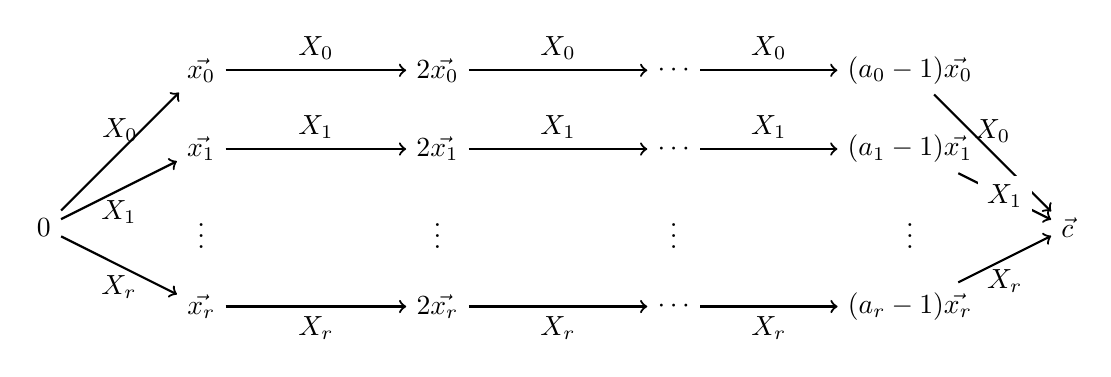
\begin{tikzpicture}[->,thick]
      \node (0) at (0,0) {0};
			\node (A1) at (2,2) {$\vec{x_0}$};
			\node (A2) at (5,2) {$2\vec{x_0}$};
      \node (A3) at (8,2) {$\cdots$};
			\node (A4) at (11,2) {$(a_0-1)\vec{x_0}$};
      \node (B1) at (2,1) {$\vec{x_1}$};
      \node (B2) at (5,1) {$2\vec{x_1}$};
      \node (B3) at (8,1) {$\cdots$};
			\node (B4) at (11,1) {$(a_1-1)\vec{x_1}$};
      \node (C1) at (2,0) {$\vdots$};
      \node (C2) at (5,0) {$\vdots$};
      \node (C3) at (8,0) {$\vdots$};
      \node (C4) at (11,0) {$\vdots$};
			\node (D1) at (2,-1) {$\vec{x_r}$};
			\node (D2) at (5,-1) {$2\vec{x_r}$};
      \node (D3) at (8,-1) {$\cdots$};
			\node (D4) at (11,-1) {$(a_r-1)\vec{x_r}$};
			\node (c) at (13,0) {$\vec{c}$};
      \draw (0) -- node[above] {$X_0$} (A1);
      \draw (A1) -- node[above] {$X_0$} (A2);
      \draw (A2) -- node[above] {$X_0$} (A3);
      \draw (A3) -- node[above] {$X_0$} (A4);
      \draw (A4) -- node[above] {$X_0$} (c);
      \draw (0) -- node[below] {$X_1$} (B1);
      \draw (B1) -- node[above] {$X_1$} (B2);
      \draw (B2) -- node[above] {$X_1$} (B3);
      \draw (B3) -- node[above] {$X_1$} (B4);
      \draw (B4) -- node[pos=.5,fill=white] {$X_1$} (c);
      \draw (0) -- node[below] {$X_r$} (D1);
      \draw (D1) -- node[below] {$X_r$} (D2);
      \draw (D2) -- node[below] {$X_r$} (D3);
      \draw (D3) -- node[below] {$X_r$} (D4);
      \draw (D4) -- node[below] {$X_r$} (c);
  \end{tikzpicture}
  \end{center}
	\[X_i^{a_i} = X_0^{a_0} - \lambda_iX_1^{a_1}.\]
	
\end{prop}

\begin{thm}[Krull--Schmidt 性]\cite{GL87}
重み付き射影直線 $\mathbb{X} $ に対して,連接層のアーベル圏
\[
\Coh(\mathbb{X}) = \qgr R_{A,\Lambda} = \gr R_{A,\Lambda}\Big{/}\tors R_{A,\Lambda}.
\]
は Krull--Schmidt 圏である.すなわち,任意の対象 $\mathcal{F} \in \Coh(\mathbb{X})$ は直既約対象の有限直和に分解でき,その分解は同型と順序を除いて一意である:
\[
\mathcal{F} \cong \bigoplus_{i=1}^n \mathcal{F}_i \quad (\text{各} \mathcal{F}_i \text{が既約対象}).
\]
\end{thm}

\begin{exmp}
$R = \CC[x, y]$ を $\ZZ$次数付き多項式環とし,$\deg(x) = 1$,$\deg(y) = 2$ とする.このとき,$R$ は重み付き射影直線 $\mathbb{P}(1,2)$ に対応し,次のような圏同値が成り立つ:
\[
\qgr R := \gr R / \tors R \simeq \Coh(\mathbb{P}(1,2)).
\]
\[
R := \CC[x, y], \quad \deg(x) = 1,\quad \deg(y) = 2.
\]

各\(n \in \ZZ_{\ge 0}\) に対して次数成分 \(R_n\) は次のように与えられる:
\[
\begin{aligned}
R_0 &= \CC \\
R_1 &= \CC x \\
R_2 &= \CC x^2 \oplus \CC y \\
R_3 &= \CC x^3 \oplus \CC x y \\
R_4 &= \CC x^4 \oplus \CC x^2 y \oplus \CC y^2 \\
&\vdots 
\end{aligned}
\]

このとき,次の列
\[
(\mathcal{O},\ \mathcal{O}(1),\ \mathcal{O}(2)),
\]
は \(\D^b(\Coh(\mathbb{P}(1,2)))\) における強例外生成列(\ref{defn:strong exceptional collection})であり,その直和
\[
T := \mathcal{O} \oplus \mathcal{O}(1) \oplus \mathcal{O}(2),
\]
は傾斜対象(\ref{defn:tilting object})となる.したがって,導来函手
\[
\RHom(T, -) \colon \D^b(\Coh(\mathbb{P}(1,2))) \longrightarrow \D^b(\mod \End(T)).
\]
は三角同値を与える.
\end{exmp}

